Converting the Iterative FFT algorithm into a parallel implementation is straight-forward. At each of the $\log N$ levels of the execution tree, there will be work that can be done in parallel. The figure below shows the combinational circuit with three stages of work, where the work done in each stage can be done in parallel.

As shown in the following figure, and seen from the previous recursion tree, a parallel implementation of the FFT algorithm can be computed in $\mathcal{O}(\log N)$ time with $N$ processors. Since no extraneous work is performed, the work complexity is $\mathcal{O}(N\log N)$, so this is a work-optimal algorithm. 

\begin{figure}[h]
\center
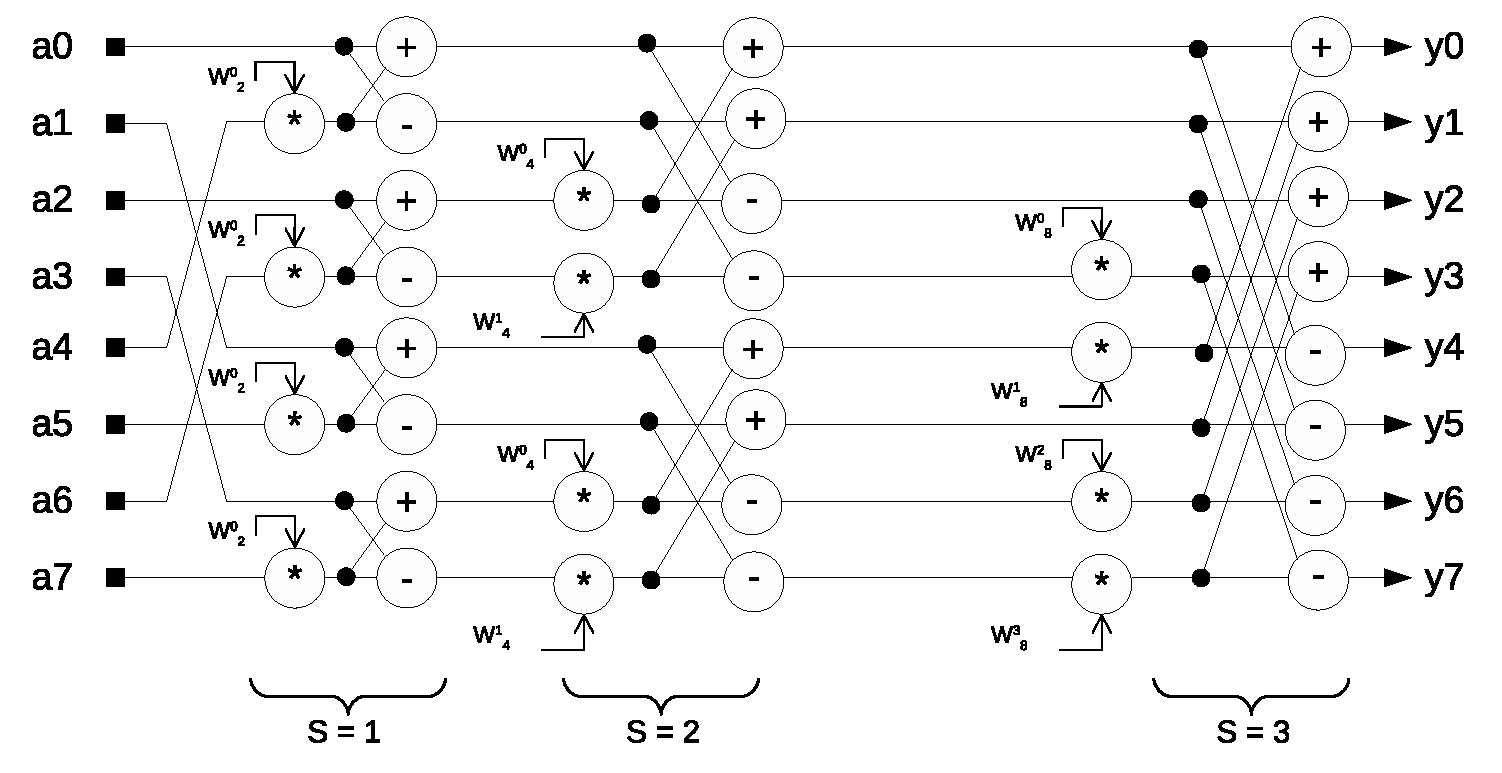
\includegraphics[scale=0.45]{img/parallel_fft_circuit.eps}
\caption{Combinational circuit Parallel-FFT that computes the FFT, here with $N=8$ inputs. The stages are labeled to correspond with the outermost loop of \texttt{FFT\_ITER()}. An FFT on $N$ inputs can be computed in $\mathcal{O}(\log N)$ depth with $\mathcal{O}(N \log N)$ elements}
\end{figure}